\documentclass{article}

\usepackage{lipsum}
\usepackage{project_440_550}
% Please submit it as is here, with line numbers.
% If you'd like a "less draft"-looking version for your website or something after:
%     \usepackage[final]{project_440_550}   % keeps the footer but kills line numbers,
%     \usepackage[preprint]{project_440_550}   % removes both
\usepackage{amsmath}
\usepackage{graphicx}
\providecommand{\IfPDFManagementActiveF}[1]{#1}
\usepackage{svg}
\usepackage[utf8]{inputenc} % allow utf-8 input
\usepackage[T1]{fontenc}    % use 8-bit T1 fonts

\usepackage[USenglish]{babel}  % there's a "canadian" option, but it's an alias for USenglish,
                               % and for some reason it makes csqoutes behave differently...
\usepackage{csquotes}       % smarter handling of quotes (used by biblatex)

\usepackage{booktabs}       % professional-quality tables
\usepackage{amsfonts}       % blackboard math symbols
\usepackage{nicefrac}       % compact symbols for 1/2, etc.
\usepackage{microtype}      % microtypography
\usepackage{xcolor}         % colors
\usepackage{hyperref}       % hyperlinks
\usepackage{url}            % simple URL typesetting

% I recommend the biblatex package.
% If you hate it for some reason, though, you can use natbib instead:
% comment out this block and uncomment the next one.

\usepackage[style=authoryear,maxbibnames=30,natbib]{biblatex}
\addbibresource{refs.bib}
\renewbibmacro{in:}{}  % drops a silly "In:" from biblatex format
\DeclareDelimFormat{nameyeardelim}{\addspace} % remove a comma i dislike, doesn't matter
\DeclareNameAlias{sortname}{given-family}  % avoid kinda-weird bib printing order

%\usepackage[round]{natbib}
%\newcommand{\printbibliography}{\bibliographystyle{plainnat}\bibliography{refs}}

\usepackage{tikz}
\usetikzlibrary{shapes.geometric, positioning, fit, backgrounds, arrows.meta, decorations.pathreplacing, calc}
\usepackage[capitalize,noabbrev]{cleveref}

\newcommand{\R}{\mathbb{R}}
\newcommand{\N}{\mathbb{N}}
\newcommand{\E}{\mathbb{E}}
\newcommand{\K}{\mathcal{K}}
\newcommand{\prox}{\operatorname{prox}}

% Theorem environments
\newtheorem{theorem}{Theorem}[section]
\newtheorem{definition}{Definition}[section]
\newtheorem{lemma}{Lemma}[section]
\newtheorem{assumption}{Assumption}


\title{Benchmark on Vision Unlearning}


% The \author macro works with any number of authors. There are two commands
% used to separate the names and addresses of multiple authors: \And and \AND.
%
% Using \And between authors leaves it to LaTeX to determine where to break the
% lines. Using \AND forces a line break at that point. So, if LaTeX puts 3 of 4
% authors names on the first line, and the last on the second line, try using
% \AND instead of \And before the third author name.

\author{%
  Inzaghi Moniaga\\
  \texttt{inzaghi@student.ubc.ca}
  \And
  Kevin K Thomas\\
  \texttt{kevinktv@cs.ubc.ca}
}

\begin{document}
\maketitle
\begin{abstract}

\end{abstract}

\section{Introduction}
In the era of big data, the ability to unlearn specific data from trained models has become increasingly important for privacy reasons. 
Although retraining a model from scratch to forget data is the best approach, it is computationally expensive. This motivates the need for efficient approximate unlearning algorithms that do not require retraining. Following the 2023 NeurIPS Unlearning Competition [\cite{neurips-2023-machine-unlearning}], several new approaches have been proposed. 
This project compares their qualitative performance against the 2023 winning solution, \cite{2023-winner}, and aims to provide a survey of the different approaches.

\subsection{Problem setup}
We base our problem setup on \cite{li2025overview}. We begin with some notation and definitions. Let $Z$ be the set of all data points and $Z^*$ be the set of all possible training datasets. Let $H$ be the set of all possible hypotheses (i.e. parameters). We define
\begin{definition}[Learning Algorithm]
    A learning algorithm $A: Z^* \to H$ maps a training dataset to a hypothesis. If $D \in Z^*$, then $A(D)$ is the model obtained by training on $D$.
\end{definition}
\begin{definition}[Unlearning Algorithm]
    An unlearning algorithm $U: H \times Z^* \times Z^* \to H$ takes a trained model, the original training dataset, and a subset of data points to unlearn, and produces a new model. Specifically, if $h = A(D)$ is the model trained on $D$, and $S \subseteq D$ is the subset of data points to unlearn, then $U(h, D, S)$ is the model obtained by unlearning $S$ from $h$.
\end{definition}
Note that both $A$ and $U$ can be randomized algorithms that define a distribution over the hypothesis space $H$.

Suppose we have a training dataset $D \in Z^*$ and a subset of data points $S \subseteq D$ that we wish to unlearn. Let $D' = D \setminus S$. The goal of machine unlearning is to create an unlearning algorithm $U$ such that the distribution of $U(A(D), D, S)$ is close to the distribution of $A(D')$ (i.e. retraining the original model on the smaller dataset).
i.e.
\begin{equation}
    \Pr[A(D')] \approx \Pr[U(A(D), D, S)]
\end{equation} 
Of course, we do not have access to the true distributions so there are several metrics that have been proposed to evaluate the performance of unlearning algorithms. One common metric is based on differential privacy. (See \cite{dwork2014algorithmic} and \cite{sekhari2021remember}). The NeurIPS 2023 Unlearning Competition uses metrics based on differential privacy.

\section{Related Work}
\subsection{Masked-Small-Gradients (MSG)}
Masked-Small-Gradients (MSG) [\cite{cadet2025}]

\subsection{SCRUB}

\subsection{DELETE}

\subsection{Kaggle Winner}

\section{Description and justification of what we did}
\begin{figure}[htbp]
    \centering
    \resizebox{\textwidth}{!}{%
    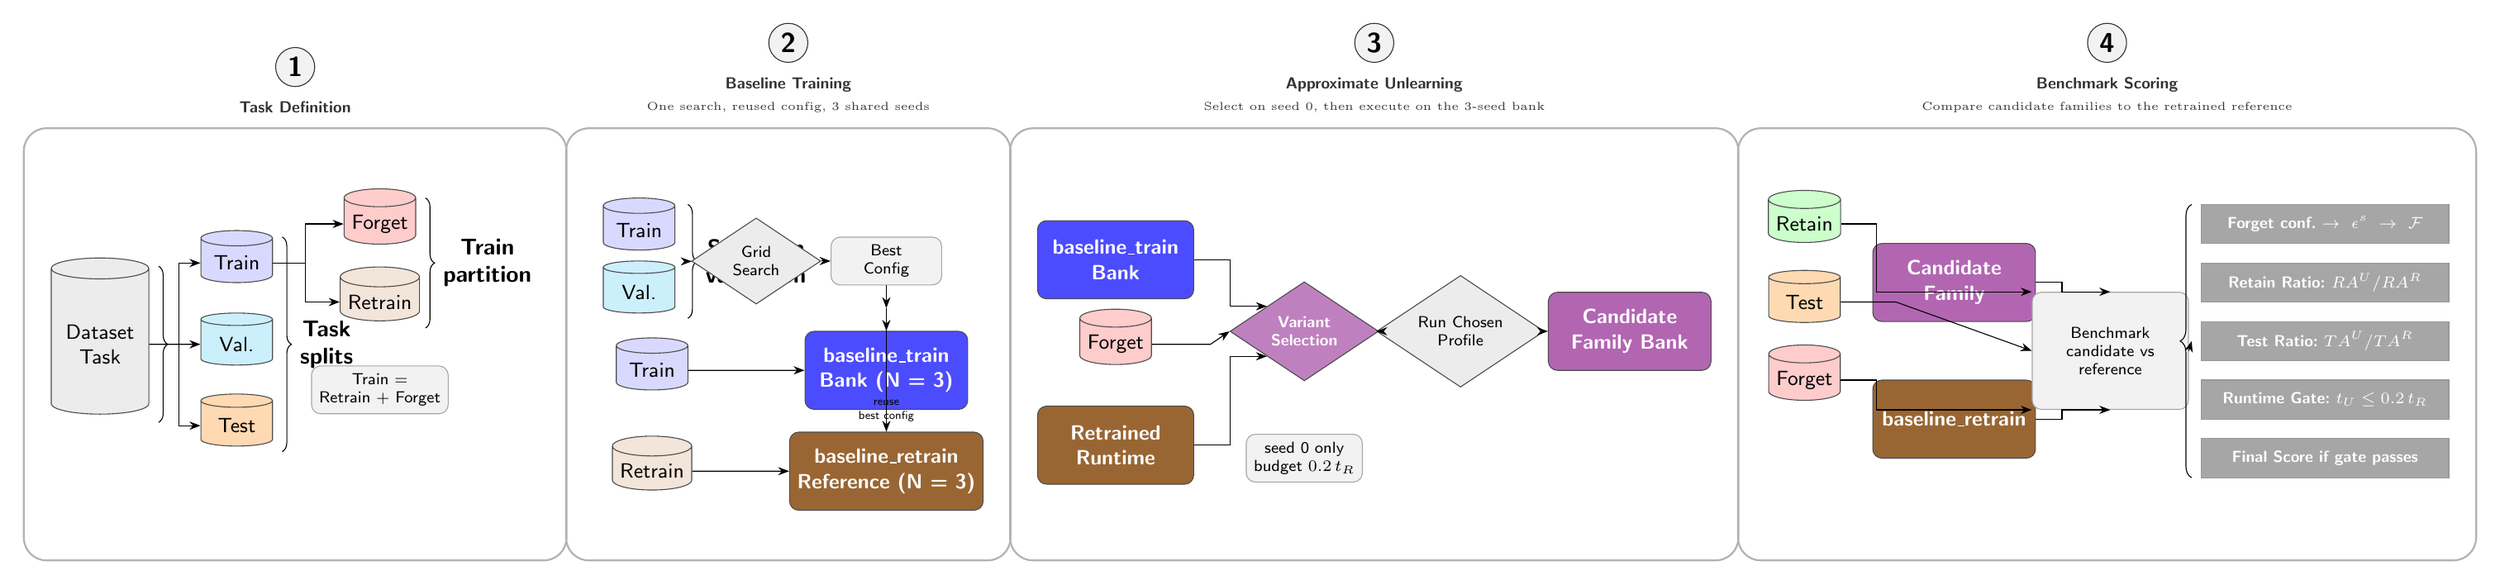
\begin{tikzpicture}[
        >=Stealth,
        font=\sffamily\small,
        db/.style={cylinder, shape border rotate=90, aspect=0.25, draw=black!70, minimum height=0.8cm, minimum width=1.1cm, align=center},
        model/.style={rectangle, rounded corners, draw=black!70, minimum height=1.2cm, minimum width=1.8cm, align=center, text=white, font=\sffamily\bfseries\small},
        action/.style={diamond, aspect=1.5, draw=black!70, minimum width=1.5cm, align=center, font=\sffamily\scriptsize},
        note/.style={rectangle, rounded corners, draw=gray!70, fill=gray!10, minimum height=0.7cm, minimum width=1.7cm, align=center, font=\sffamily\scriptsize},
        metric/.style={rectangle, draw=gray!80, fill=gray!70, text=white, minimum height=0.6cm, minimum width=3.8cm, align=center, font=\sffamily\scriptsize\bfseries},
        box/.style={rectangle, draw=gray!60, thick, rounded corners=10pt, minimum height=6.2cm, inner sep=12pt},
        hdr/.style={rectangle, align=center, fill=white, font=\sffamily\scriptsize\bfseries, text=black!80},
        circ/.style={circle, draw=black!80, font=\sffamily\large\bfseries, inner sep=2pt, minimum size=0.6cm, fill=gray!10},
        colTrain/.style={fill=blue!15, text=black},
        colRetain/.style={fill=green!20, text=black},
        colForget/.style={fill=red!20, text=black},
        colRetrainData/.style={fill=brown!20, text=black},
        colVal/.style={fill=cyan!20, text=black},
        colTest/.style={fill=orange!30, text=black},
        colOrig/.style={fill=blue!70, text=white},
        colRetrain/.style={fill=brown!80!black, text=white},
        colUnlearn/.style={fill=violet!60, text=white}
    ]

        \begin{scope}[local bounding box=phase1_inner]
            \path (0, 2.9) -- (0, -2.9);

            \node[db, fill=gray!15, minimum height=2.4cm, minimum width=1.5cm] (task_main) at (0,0) {Dataset\\Task};

            \coordinate (d_top) at ($(task_main.center) + (0.9, 1.2)$);
            \coordinate (d_bot) at ($(task_main.center) + (0.9, -1.2)$);
            \draw[decorate,decoration={brace,amplitude=4pt}] (d_top) -- (d_bot);

            \node[db, colTrain]       (db_train1)   at (2.1,  1.25) {Train};
            \node[db, colVal]         (db_val1)     at (2.1,  0.00) {Val.};
            \node[db, colTest]        (db_test1)    at (2.1, -1.25) {Test};
            \node[db, colForget]      (db_forget1)  at (4.3,  1.85) {Forget};
            \node[db, colRetrainData] (db_retrain1) at (4.3,  0.65) {Retrain};
            \node[note, minimum width=2.0cm] (db_train_note) at (4.3, -0.70) {Train =\\Retrain + Forget};

            \draw[->] (task_main.east) -- ++(0.45,0) |- (db_train1.west);
            \draw[->] (task_main.east) -- ++(0.45,0) -- (db_val1.west);
            \draw[->] (task_main.east) -- ++(0.45,0) |- (db_test1.west);
            \draw[->] (db_train1.east) -- ++(0.50,0) |- (db_forget1.west);
            \draw[->] (db_train1.east) -- ++(0.50,0) |- (db_retrain1.west);

            \coordinate (s_top) at ($(db_train1.center) + (0.7, 0.4)$);
            \coordinate (s_bot) at ($(db_test1.center) + (0.7, -0.4)$);
            \draw[decorate,decoration={brace,amplitude=4pt}] (s_top) -- (s_bot) 
                node[midway, right=0.15cm, align=center, font=\sffamily\bfseries] {Task\\splits};

            \coordinate (t_top) at ($(db_forget1.center) + (0.7, 0.4)$);
            \coordinate (t_bot) at ($(db_retrain1.center) + (0.7, -0.4)$);
            \draw[decorate,decoration={brace,amplitude=4pt}] (t_top) -- (t_bot)
                node[midway, right=0.15cm, align=center, font=\sffamily\bfseries] {Train\\partition};
        \end{scope}

        \node[box, fit=(phase1_inner)] (box1) {};
        \node[hdr, above=0.1cm of box1] (hdr1) {Task Definition};
        \node[circ, above=0.1cm of hdr1] {1};


        \begin{scope}[shift={(box1.east)}, xshift=0.4cm, local bounding box=phase2_inner]
            \path (0, 2.9) -- (0, -2.9);

            \node[db, colTrain] (p2_train_search) at (0.7,  1.75) {Train};
            \node[db, colVal]   (p2_val_search)   at (0.7,  0.80) {Val.};
            \coordinate (p2_s_top) at ($(p2_train_search.center) + (0.75, 0.4)$);
            \coordinate (p2_s_bot) at ($(p2_val_search.center) + (0.75, -0.4)$);
            \draw[decorate,decoration={brace,amplitude=4pt}] (p2_s_top) -- (p2_s_bot)
                node[midway, right=0.15cm, align=center, font=\sffamily\bfseries] {Select on\\validation};

            \node[action, fill=gray!15] (p2_search) at (2.5, 1.28) {Grid\\Search};
            \node[note] (p2_cfg) at (4.5, 1.28) {Best\\Config};
            \draw[->] ($(p2_s_top)!0.5!(p2_s_bot) + (0.05, 0)$) -- (p2_search);
            \draw[->] (p2_search) -- (p2_cfg);

            \node[db, colTrain]       (p2_train_run)   at (0.9, -0.40) {Train};
            \node[model, colOrig, minimum width=2.5cm] (p2_train_bank) at (4.5, -0.40) {baseline\_train\\Bank (N = 3)};
            \draw[->] (p2_train_run.east) -- (p2_train_bank.west);

            \node[db, colRetrainData] (p2_retrain_run) at (0.9, -1.95) {Retrain};
            \node[model, colRetrain, minimum width=2.5cm] (p2_retrain_bank) at (4.5, -1.95) {baseline\_retrain\\Reference (N = 3)};
            \draw[->] (p2_retrain_run.east) -- (p2_retrain_bank.west);

            \coordinate (p2_cfg_split) at ($(p2_cfg.south) + (0, -0.35)$);
            \draw[->] (p2_cfg.south) -- (p2_cfg_split);
            \draw[->] (p2_cfg_split) -| (p2_train_bank.north);
            \draw[->] (p2_cfg_split) -| (p2_retrain_bank.north);
            \node[font=\sffamily\tiny, align=center] at ($(p2_retrain_bank.north) + (0, 0.32)$) {reuse\\best config};
        \end{scope}

        \node[box, fit=(phase2_inner)] (box2) {};
        \node[hdr, above=0.1cm of box2] (hdr2) {Baseline Training\\[0.5ex] \normalfont\tiny One search, reused config, 3 shared seeds};
        \node[circ, above=0.1cm of hdr2] {2};


        \begin{scope}[shift={(box2.east)}, xshift=0.4cm, local bounding box=phase3_inner]
            \path (0, 2.9) -- (0, -2.9);

            \node[model, colOrig, minimum width=2.4cm] (p3_base) at (1.2,  1.30) {baseline\_train\\Bank};
            \node[db, colForget] (p3_forget) at (1.2, 0.00) {Forget};
            \node[model, colRetrain, minimum width=2.4cm] (p3_ref) at (1.2, -1.55) {Retrained\\Runtime};

            \node[action, fill=violet!50, text=white, font=\sffamily\scriptsize\bfseries] (p3_select) at (4.1, 0.20) {Variant\\Selection};
            \node[note] (p3_budget) at (4.1, -1.75) {seed 0 only\\budget $0.2\,t_R$};
            \node[action, fill=gray!15] (p3_run) at (6.5, 0.20) {Run Chosen\\Profile};
            \node[model, colUnlearn, minimum width=2.5cm] (p3_candidate) at (9.1, 0.20) {Candidate\\Family Bank};

            \draw[->] (p3_base.east) -- ++(0.55,0) |- (p3_select.north west);
            \draw[->] (p3_forget.east) -- ++(0.90,0) -- (p3_select.west);
            \draw[->] (p3_ref.east) -- ++(0.55,0) |- (p3_select.south west);
            \draw[->] (p3_select) -- (p3_run);
            \draw[->] (p3_run) -- (p3_candidate);
        \end{scope}

        \node[box, fit=(phase3_inner)] (box3) {};
        \node[hdr, above=0.1cm of box3] (hdr3) {Approximate Unlearning\\[0.5ex] \normalfont\tiny Select on seed 0, then execute on the 3-seed bank};
        \node[circ, above=0.1cm of hdr3] {3};


        \begin{scope}[shift={(box3.east)}, xshift=0.4cm, local bounding box=phase4_inner]
            \path (0, 2.9) -- (0, -2.9);

            \node[db, colRetain] (p4_retain) at (0.6,  1.85) {Retain};
            \node[db, colTest]   (p4_test)   at (0.6,  0.65) {Test};
            \node[db, colForget] (p4_forget) at (0.6, -0.55) {Forget};

            \node[model, colUnlearn, minimum width=2.5cm] (p4_candidate) at (2.9,  0.95) {Candidate\\Family};
            \node[model, colRetrain, minimum width=2.5cm] (p4_reference) at (2.9, -1.15) {baseline\_retrain};
            \node[note, minimum width=2.4cm, minimum height=1.8cm] (p4_compare) at (5.3, -0.10) {Benchmark\\candidate vs\\reference};

            \draw[->] (p4_retain.east) -- ++(0.55,0) |- (p4_compare.north west);
            \draw[->] (p4_test.east) -- ++(0.85,0) -- (p4_compare.west);
            \draw[->] (p4_forget.east) -- ++(0.55,0) |- (p4_compare.south west);
            \draw[->] (p4_candidate.east) -- ++(0.40,0) |- (p4_compare.north);
            \draw[->] (p4_reference.east) -- ++(0.40,0) |- (p4_compare.south);

            \node[metric] (m1) at (8.6,  1.85) {Forget conf.\ $\rightarrow\ \epsilon^s\ \rightarrow\ \mathcal{F}$};
            \node[metric] (m2) at (8.6,  0.95) {Retain Ratio:\ $RA^U/RA^R$};
            \node[metric] (m3) at (8.6,  0.05) {Test Ratio:\ $TA^U/TA^R$};
            \node[metric] (m4) at (8.6, -0.85) {Runtime Gate:\ $t_U \leq 0.2\,t_R$};
            \node[metric] (m5) at (8.6, -1.75) {Final Score if gate passes};

            \coordinate (m_left_top) at (6.55, 2.15);
            \coordinate (m_left_bot) at (6.55, -2.05);
            \draw[decorate,decoration={brace,amplitude=5pt,mirror}] (m_left_top) -- (m_left_bot) coordinate[midway] (p4_metric_mid);
            \draw[->] (p4_compare.east) -- (p4_metric_mid);
        \end{scope}

        \node[box, fit=(phase4_inner)] (box4) {};
        \node[hdr, above=0.1cm of box4] (hdr4) {Benchmark Scoring\\[0.5ex] \normalfont\tiny Compare candidate families to the retrained reference};
        \node[circ, above=0.1cm of hdr4] {4};

    \end{tikzpicture}%
    }
    \caption{Pipeline used for each dataset-task benchmark. Phase 1 constructs a manifest-defined task with named \texttt{train}, \texttt{val}, and \texttt{test} splits, where the canonical \texttt{train} split is further partitioned as \texttt{train} $=$ \texttt{retrain} $+$ \texttt{forget}. Phase 2 runs one small validation-based grid search on the \texttt{train} split, keeps the best configuration, and reuses it to train matched \texttt{baseline\_train} and \texttt{baseline\_retrain} seed banks over the same three random initializations. Phase 3 applies each approximate unlearning family starting from \texttt{baseline\_train}; when efficiency-aware execution is enabled, a reduced variant is selected on the first seed under the runtime budget $0.2\,t_R$ derived from the retrained reference, and the selected profile is then run across the full three-seed bank. Phase 4 benchmarks \texttt{baseline\_train} and each unlearning family against \texttt{baseline\_retrain} on the retain, test, and forget splits, computing forgetting quality from per-example epsilons and combining it with retain and test accuracy ratios, with the final score kept only if the runtime cutoff is satisfied.}
    \label{fig:pipeline}
\end{figure}

Figure~\ref{fig:pipeline} summarizes the benchmark pipeline we implemented. Each experiment begins from a manifest-defined task with \texttt{train}, \texttt{val}, and \texttt{test} splits, where \texttt{train} is explicitly partitioned into the disjoint \texttt{forget} and \texttt{retrain} subsets. For a given dataset, we run one small validation-based grid search on \texttt{train}, keep the best configuration, and then reuse that same configuration to build two matched three-seed banks: \texttt{baseline\_train}, trained on \texttt{train}, and \texttt{baseline\_retrain}, trained from scratch on \texttt{retrain} and used as the reference family.

This design keeps the comparison controlled and practical. Every approximate unlearning method starts from the same \texttt{baseline\_train} checkpoints and the same \texttt{forget} split, and the efficiency-aware selection step uses one seed to choose a variant that respects the retraining budget before the selected profile is executed across all three seeds. We then score \texttt{baseline\_train} and every unlearning family against \texttt{baseline\_retrain} using the implemented product $\mathcal{F} \times \frac{RA^U}{RA^R} \times \frac{TA^U}{TA^R}$, while only keeping that score when the runtime condition $t_U \leq 0.2\,t_R$ holds.

\section{Experiment Setup}
In our experiments, we benchmark several approximate machine unlearning algorithms against a gold-standard baseline (retraining from scratch). For our base architecture, we utilize a randomly initialized ResNet-18 model with no pre-trained weights. To ensure optimal performance, we independently tune hyperparameters for each dataset via a small grid search on a dedicated validation set. Full details of this tuning process can be found in \Cref{fig:hyperparameterTuning}.

% To accommodate smaller image resolutions without suffering from spatial detail collapse, the ResNet-18 stem is modified for $32 \times 32$ inputs by replacing the initial $7 \times 7$ convolution with a $3 \times 3$ kernel and swapping the max-pooling layer with an identity mapping. For larger inputs, the standard ResNet-18 stem is preserved.

\subsection{Dataset}

We evaluate the unlearning algorithms across three primary image classification datasets: Kaggle Machine Unlearning Dataset \citep{neurips-2023-machine-unlearning}, CIFAR-10 \citep{Krizhevsky09learningmultiple}, MUFAC \citep{choi2023machine}.

For the unlearning task, the canonical training partition is deterministically divided into two mutually exclusive sets:
\begin{enumerate}
    \item \textbf{Forget Set ($S$):} A subset of the training data selected to be unlearned. Our generation pipeline builds a mixed-label unlearning task that proportionally targets specific classes or targets a globally defined forget percentage.
    \item \textbf{Retain Set ($D \setminus S$):} The remaining data from the training partition, representing the data the model must preserve.
\end{enumerate}

Held-out validation and test sets are strictly maintained to measure generalization during unlearning.

\begin{figure}[htbp]
    \centering
    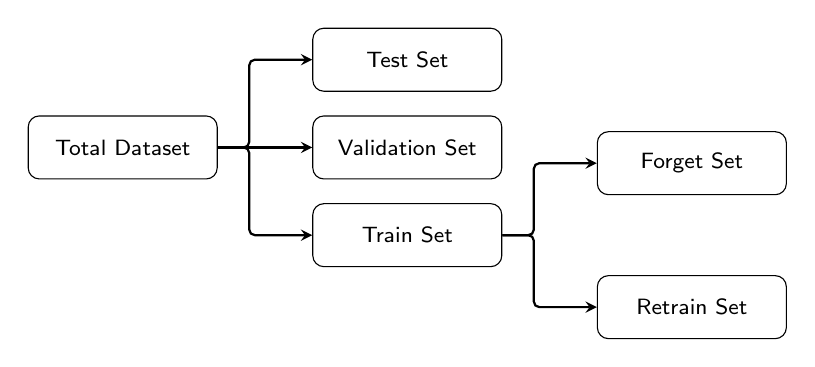
\begin{tikzpicture}[
        node distance=0.4cm and 1.5cm,
        box/.style={draw, rectangle, rounded corners, align=center, minimum width=2.4cm, minimum height=0.8cm, font=\sffamily\footnotesize},
        arrow/.style={->, >=stealth, thick, rounded corners=2pt}
    ]

    % Top Level Dataset
    \node[box] (dataset) {Total Dataset};

    % Level 1: Direct 3-way split
    \node[box] (val) [right=1.2cm of dataset] {Validation Set};
    \node[box] (test) [above=0.3cm of val] {Test Set};
    \node[box] (train) [below=0.3cm of val] {Train Set};

    % Level 2: Unlearning splits from Train
    \node[box] (forget) [above right=0.1cm and 1.2cm of train] {Forget Set};
    \node[box] (retrain) [below right=0.1cm and 1.2cm of train] {Retrain Set};

    % Edges from Total Dataset
    \draw [arrow] (dataset.east) -- +(0.4,0) |- (test.west);
    \draw [arrow] (dataset.east) -- (val.west);
    \draw [arrow] (dataset.east) -- +(0.4,0) |- (train.west);

    % Edges from Train Set
    \draw [arrow] (train.east) -- +(0.4,0) |- (forget.west);
    \draw [arrow] (train.east) -- +(0.4,0) |- (retrain.west);

    \end{tikzpicture}
    \vspace{-0.5em}
    \caption{Data partitioning pipeline for unlearning tasks. The dataset is first divided into test, validation, and training sets. The training data is further partitioned into a \textit{forget set} (target samples to be unlearned) and a disjoint \textit{retrain set} (used to train clean baseline models from scratch).}
    \label{fig:dataset_splits}
\end{figure}

\subsection{Evaluation}
To strictly evaluate the qualitative performance of the approximate unlearning methods, we utilize an extensive benchmark pipeline that directly follows the \textbf{NeurIPS 2023 Machine Unlearning Competition} methodology \citep{neurips-2023-machine-unlearning}.

The evaluation protocol tests the algorithms over predefined seed banks and enforces a hard time-efficiency threshold. The performance is quantified through a four-step calculation:

\subsubsection*{Step 1: Estimating Per-Example Indistinguishability ($\epsilon^s$)}
Because it is computationally intractable to measure exact indistinguishability for the entire model, the evaluation estimates an $\epsilon$ value for each individual example $s$ in the forget set $S$. We apply various ``attacks'' on the model outputs to distinguish unlearned models from retrained baselines, generating a False Positive Rate (FPR) and a False Negative Rate (FNR). For each attack, the privacy parameters are estimated as:
\begin{align}
    \epsilon_1 &= \log(1 - \delta - \text{FPR}) - \log(\text{FNR}) \\
    \epsilon_2 &= \log(1 - \delta - \text{FNR}) - \log(\text{FPR})
\end{align}
The final $\epsilon^s$ for that specific example is derived from the maximum value (representing the worst-case, strongest attack):
\begin{equation}
    \epsilon^s = \max(\epsilon_1, \epsilon_2)
\end{equation}

\subsubsection*{Step 2: Calculating Forgetting Quality ($\mathcal{F}$)}
Once $\epsilon^s$ is calculated, it is mapped to a scoring function $\mathcal{H}(s)$. The function places the $\epsilon^s$ value into a predefined ``bin'' indexed as $n(s)$. The assigned score decays exponentially as the required $\epsilon$ bound increases:
\begin{equation}
    \mathcal{H}(s) = \frac{2}{2^{n(s)}}
\end{equation}
The total forgetting quality, $\mathcal{F}$, is defined as the average of these scores across all examples in the forget set:
\begin{equation}
    \mathcal{F} = \frac{1}{|S|} \sum_{s \in S} \mathcal{H}(s)
\end{equation}

\subsubsection*{Step 3: Calculating Model Utility}
An unlearning algorithm is only viable if the model retains its core predictive utility. Utility is defined by the accuracy of a set of models $O$ on two disjoint datasets: the retain set ($D \setminus S$) and a held-out test set ($T$). 
\begin{align}
    \text{Retain Accuracy (RA)}&: \quad RA(O) = \frac{1}{|O|} \sum_{i=1}^{|O|} Acc(O_i, D \setminus S) \\
    \text{Test Accuracy (TA)}&: \quad TA(O) = \frac{1}{|O|} \sum_{i=1}^{|O|} Acc(O_i, T)
\end{align}
We compute these average accuracies for the candidate unlearned models ($RA^U$ and $TA^U$) and compare them directly against the ideal retrained models ($RA^R$ and $TA^R$).

\subsubsection*{Step 4: The Final Combined Score}
Unlearning algorithms must first pass a hard threshold for time efficiency (operating strictly faster than the time required for full retraining). If the candidate passes the efficiency cutoff, the mathematical components are combined into a final performance score:
\begin{equation}
    \text{Score} = \mathcal{F} \times \frac{RA^U}{RA^R} \times \frac{TA^U}{TA^R}
\end{equation}
This final formulation scales the forgetting quality $\mathcal{F}$ by the utility ratios. It explicitly penalizes the score if the unlearned model performs worse than the perfectly retrained model on the retain or test distributions. The resulting score is strictly bounded in the range $[0, 1]$:
\begin{itemize}
    \item A score approaching \textbf{1.0} indicates a flawless unlearner that seamlessly mimics a retrained model without utility loss.
    \item A score approaching \textbf{0.0} signifies that the algorithm either failed to effectively forget the targeted data, completely collapsed the model's accuracy, or failed the runtime efficiency requirements.
\end{itemize}


\section{Discussion and future work}

The benchmark results show that \textbf{MSG} is the only method that remains competitive across both datasets when forgetting quality, utility retention, and runtime are combined into a single score. It achieves the best final score on CIFAR-10 ($0.2646$) and MUFAC ($0.2742$), while running roughly $8.0\times$ and $9.4\times$ faster than retraining, respectively. Its retain accuracy remains very close to the retrained reference on both datasets, and its test accuracy changes only modestly, making it the most balanced unlearning method in our study. \Cref{fig:benchmarkTradeoffs} also highlights an important property of the evaluation itself: the \texttt{baseline\_train} family still attains nonzero raw scores ($0.2120$ on CIFAR-10 and $0.0850$ on MUFAC), but it fails the efficiency cutoff and is therefore disqualified. This is desirable, because the benchmark is intended to reward practical unlearning rather than strong accuracy alone.

\begin{figure}[htbp]
    \centering
    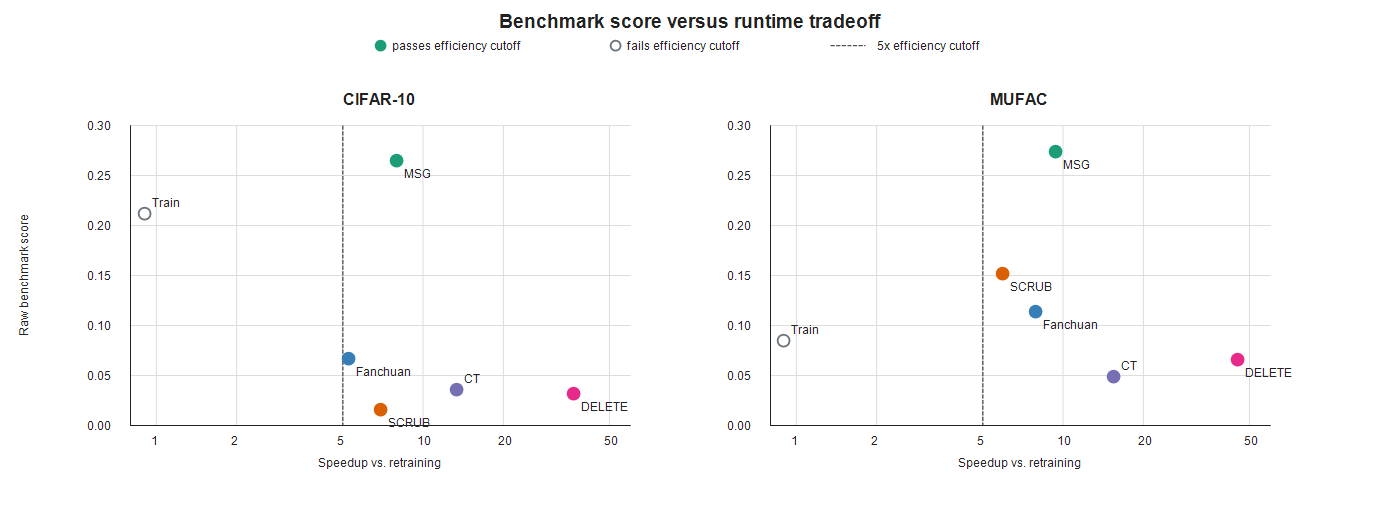
\includegraphics[width=1\linewidth]{figures/benchmark-score-speedup.png}
    \caption{Raw benchmark score versus speedup over retraining for each model family. The dashed vertical line marks the $5\times$ speedup implied by the efficiency cutoff. Filled points pass the cutoff, while the hollow training baseline remains disqualified despite a nonzero raw score.}
    \label{fig:benchmarkTradeoffs}
\end{figure}

The remaining methods each expose a different failure mode. \textbf{FanchuanUnlearning} preserves utility almost perfectly, but its forgetting quality is too weak to compete, yielding final scores of only $0.0667$ on CIFAR-10 and $0.1139$ on MUFAC despite solid speedups. \textbf{SCRUB} is much more dataset-sensitive: it performs poorly on CIFAR-10, but on MUFAC it reaches the second-best final score ($0.1522$) and the highest test accuracy ($0.5000$), while still suffering a large retain-accuracy drop to $0.6265$. This makes SCRUB interesting, but unstable. At the other extreme, \textbf{CT} and \textbf{DELETE} are the fastest methods in the benchmark, reaching roughly $13\times$ to $45\times$ speedups, yet their retain and test accuracies fall too far below retraining to remain competitive on the final score. Taken together, these comparisons suggest that fast approximate unlearning is not enough by itself; the strongest methods are the ones that preserve utility while still producing a meaningful privacy-oriented forgetting signal.

Several limitations of our current study point directly to future work. We only evaluate two datasets, one forget-task construction (\texttt{forget\_mixed}), and three models per family, so the robustness of the ranking is still limited. A natural next step is to test additional forget-set structures, such as class-specific, random, or long-tail deletion tasks, and to increase the number of seeds so that dataset-specific volatility can be measured more reliably. It would also be useful to retune each unlearning algorithm more aggressively rather than relying on a single shared experimental envelope, since methods like SCRUB appear especially sensitive to dataset characteristics. Finally, extending the benchmark beyond a randomly initialized ResNet-18 and complementing the hard runtime cutoff with Pareto-style or cost-aware analyses would give a more complete view of when a method is genuinely preferable to retraining.


\printbibliography


%%%%%%%%%%%%%%%%%%%%%%%%%%%%%%%%%%%%%%%%%%%%%%%%%%%%%%%%%%%%
\newpage
\appendix

\section{Supplementary material} \label{app:info}

This stuff doesn't count towards your page limit.

\begin{figure}[htbp]
    \centering
    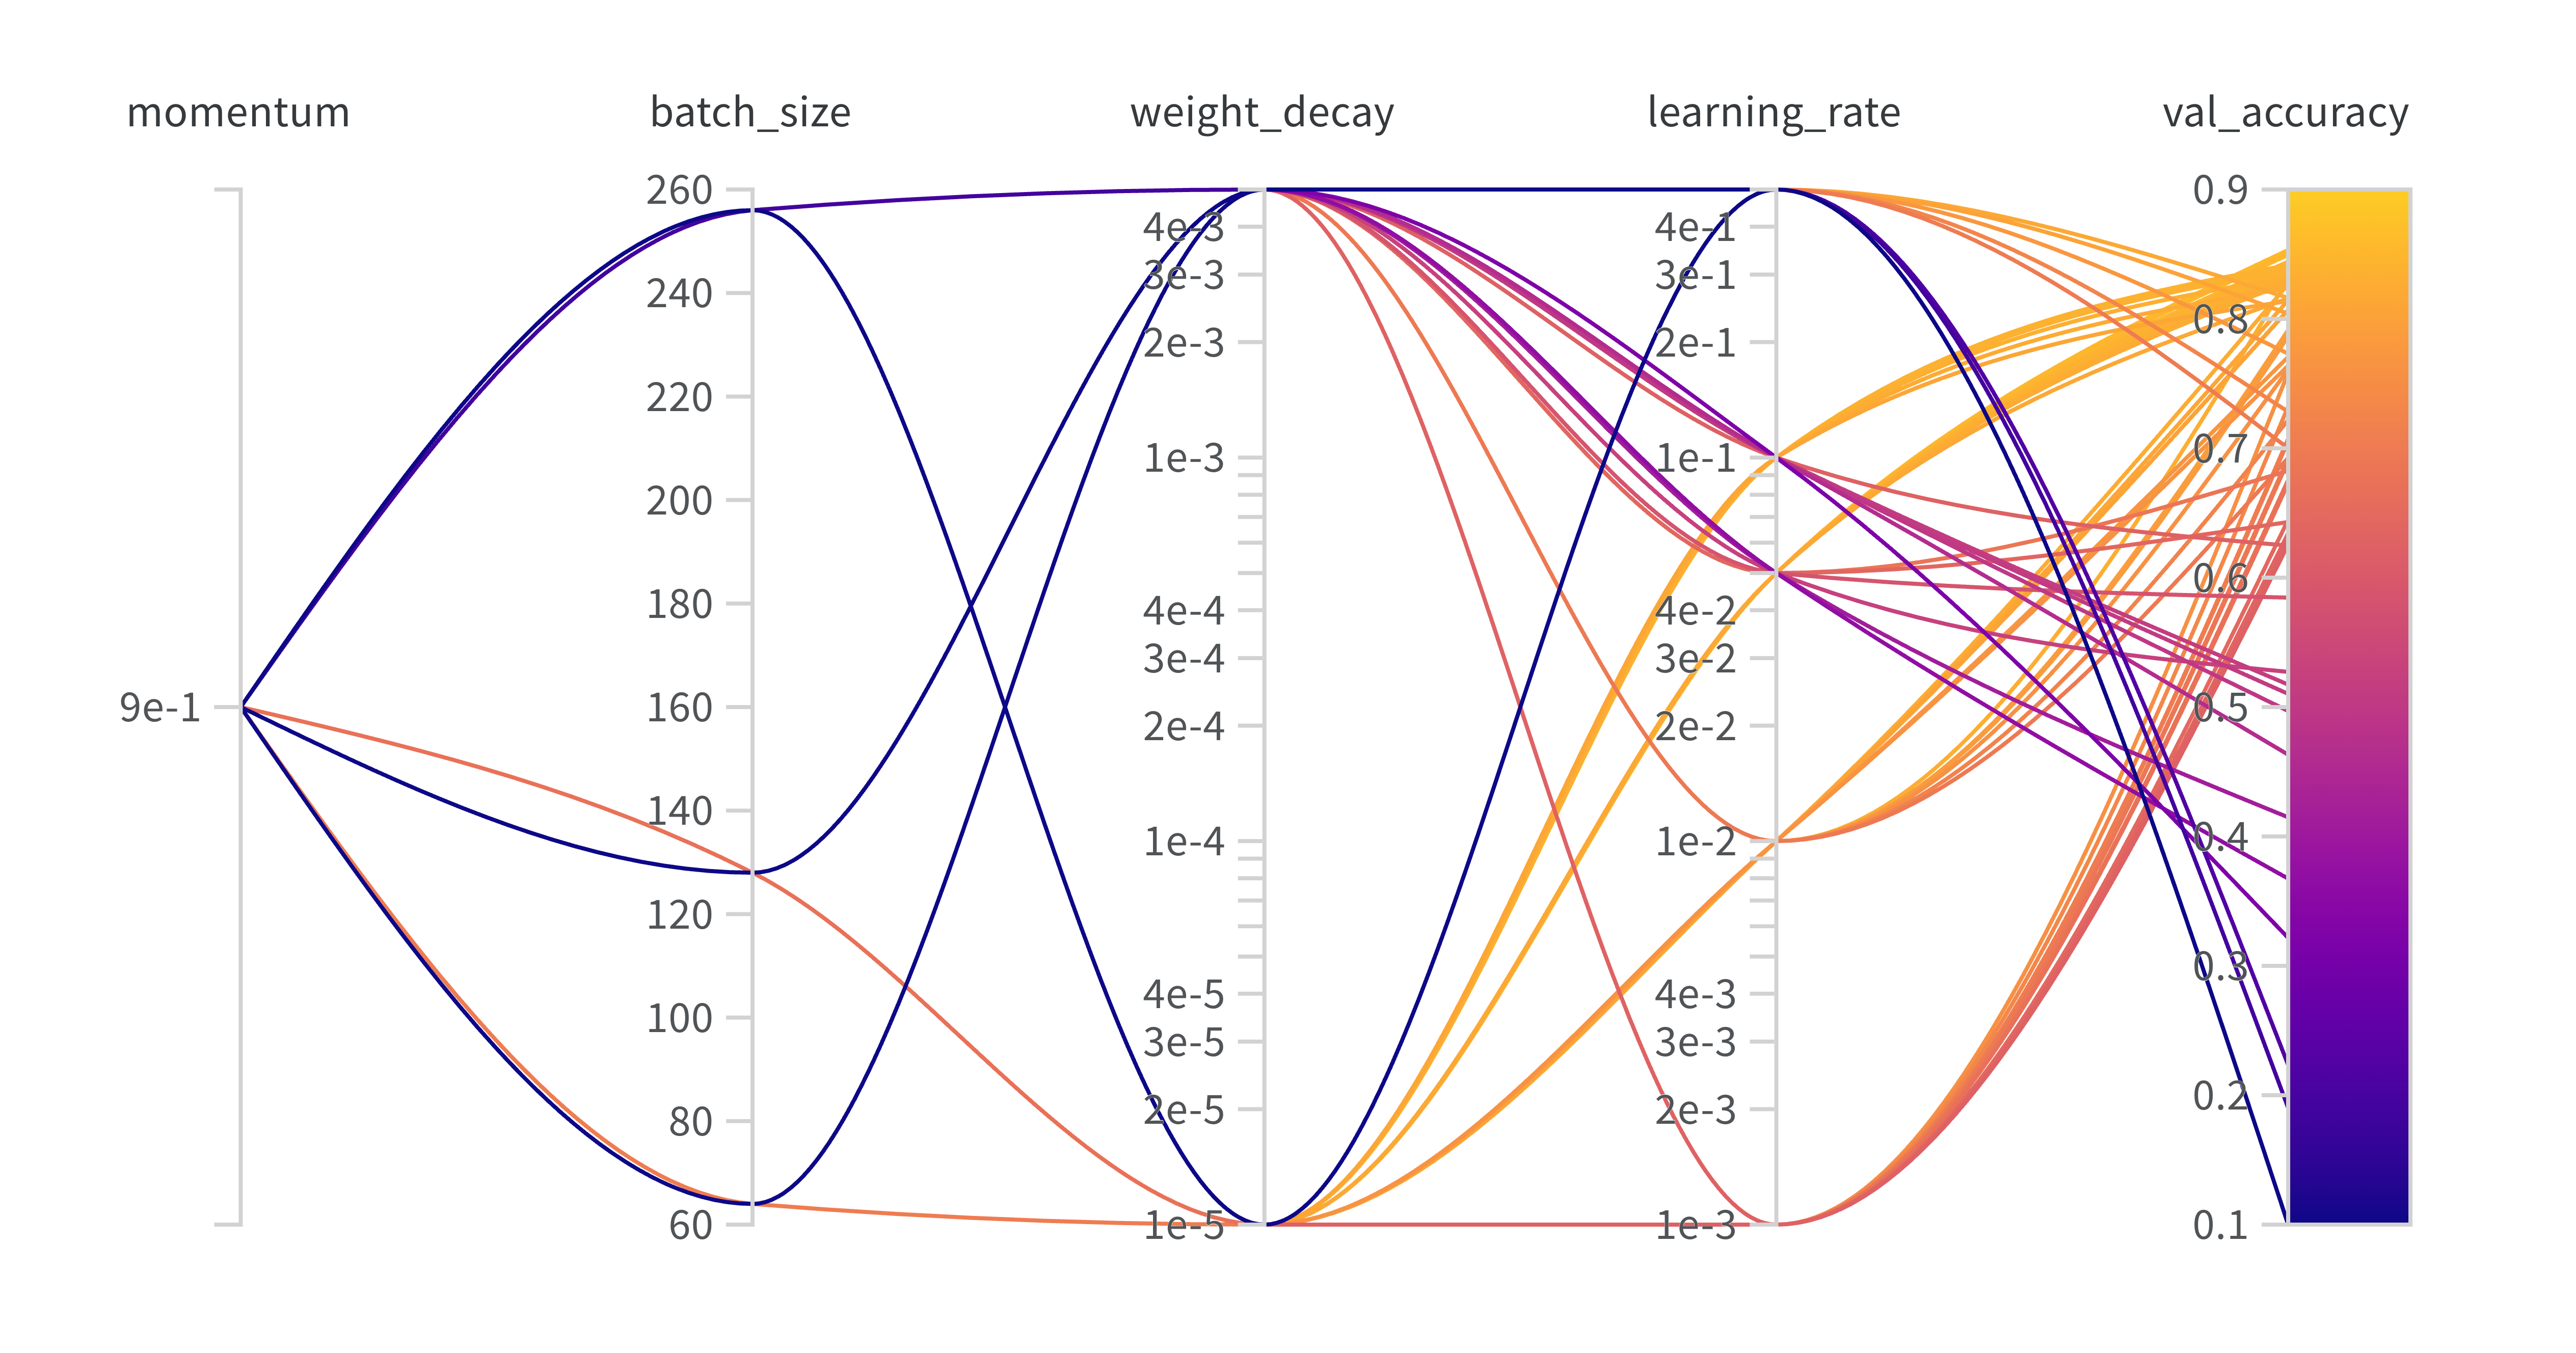
\includegraphics[width=1\linewidth]{figures/cifar-hyperparameter-tuning.png}
    \caption{Cifar-10 Hyperparmeter tuning for Resnet18}
    \label{fig:hyperparameterTuning}
\end{figure}

\begin{figure}[htbp]
    \centering
    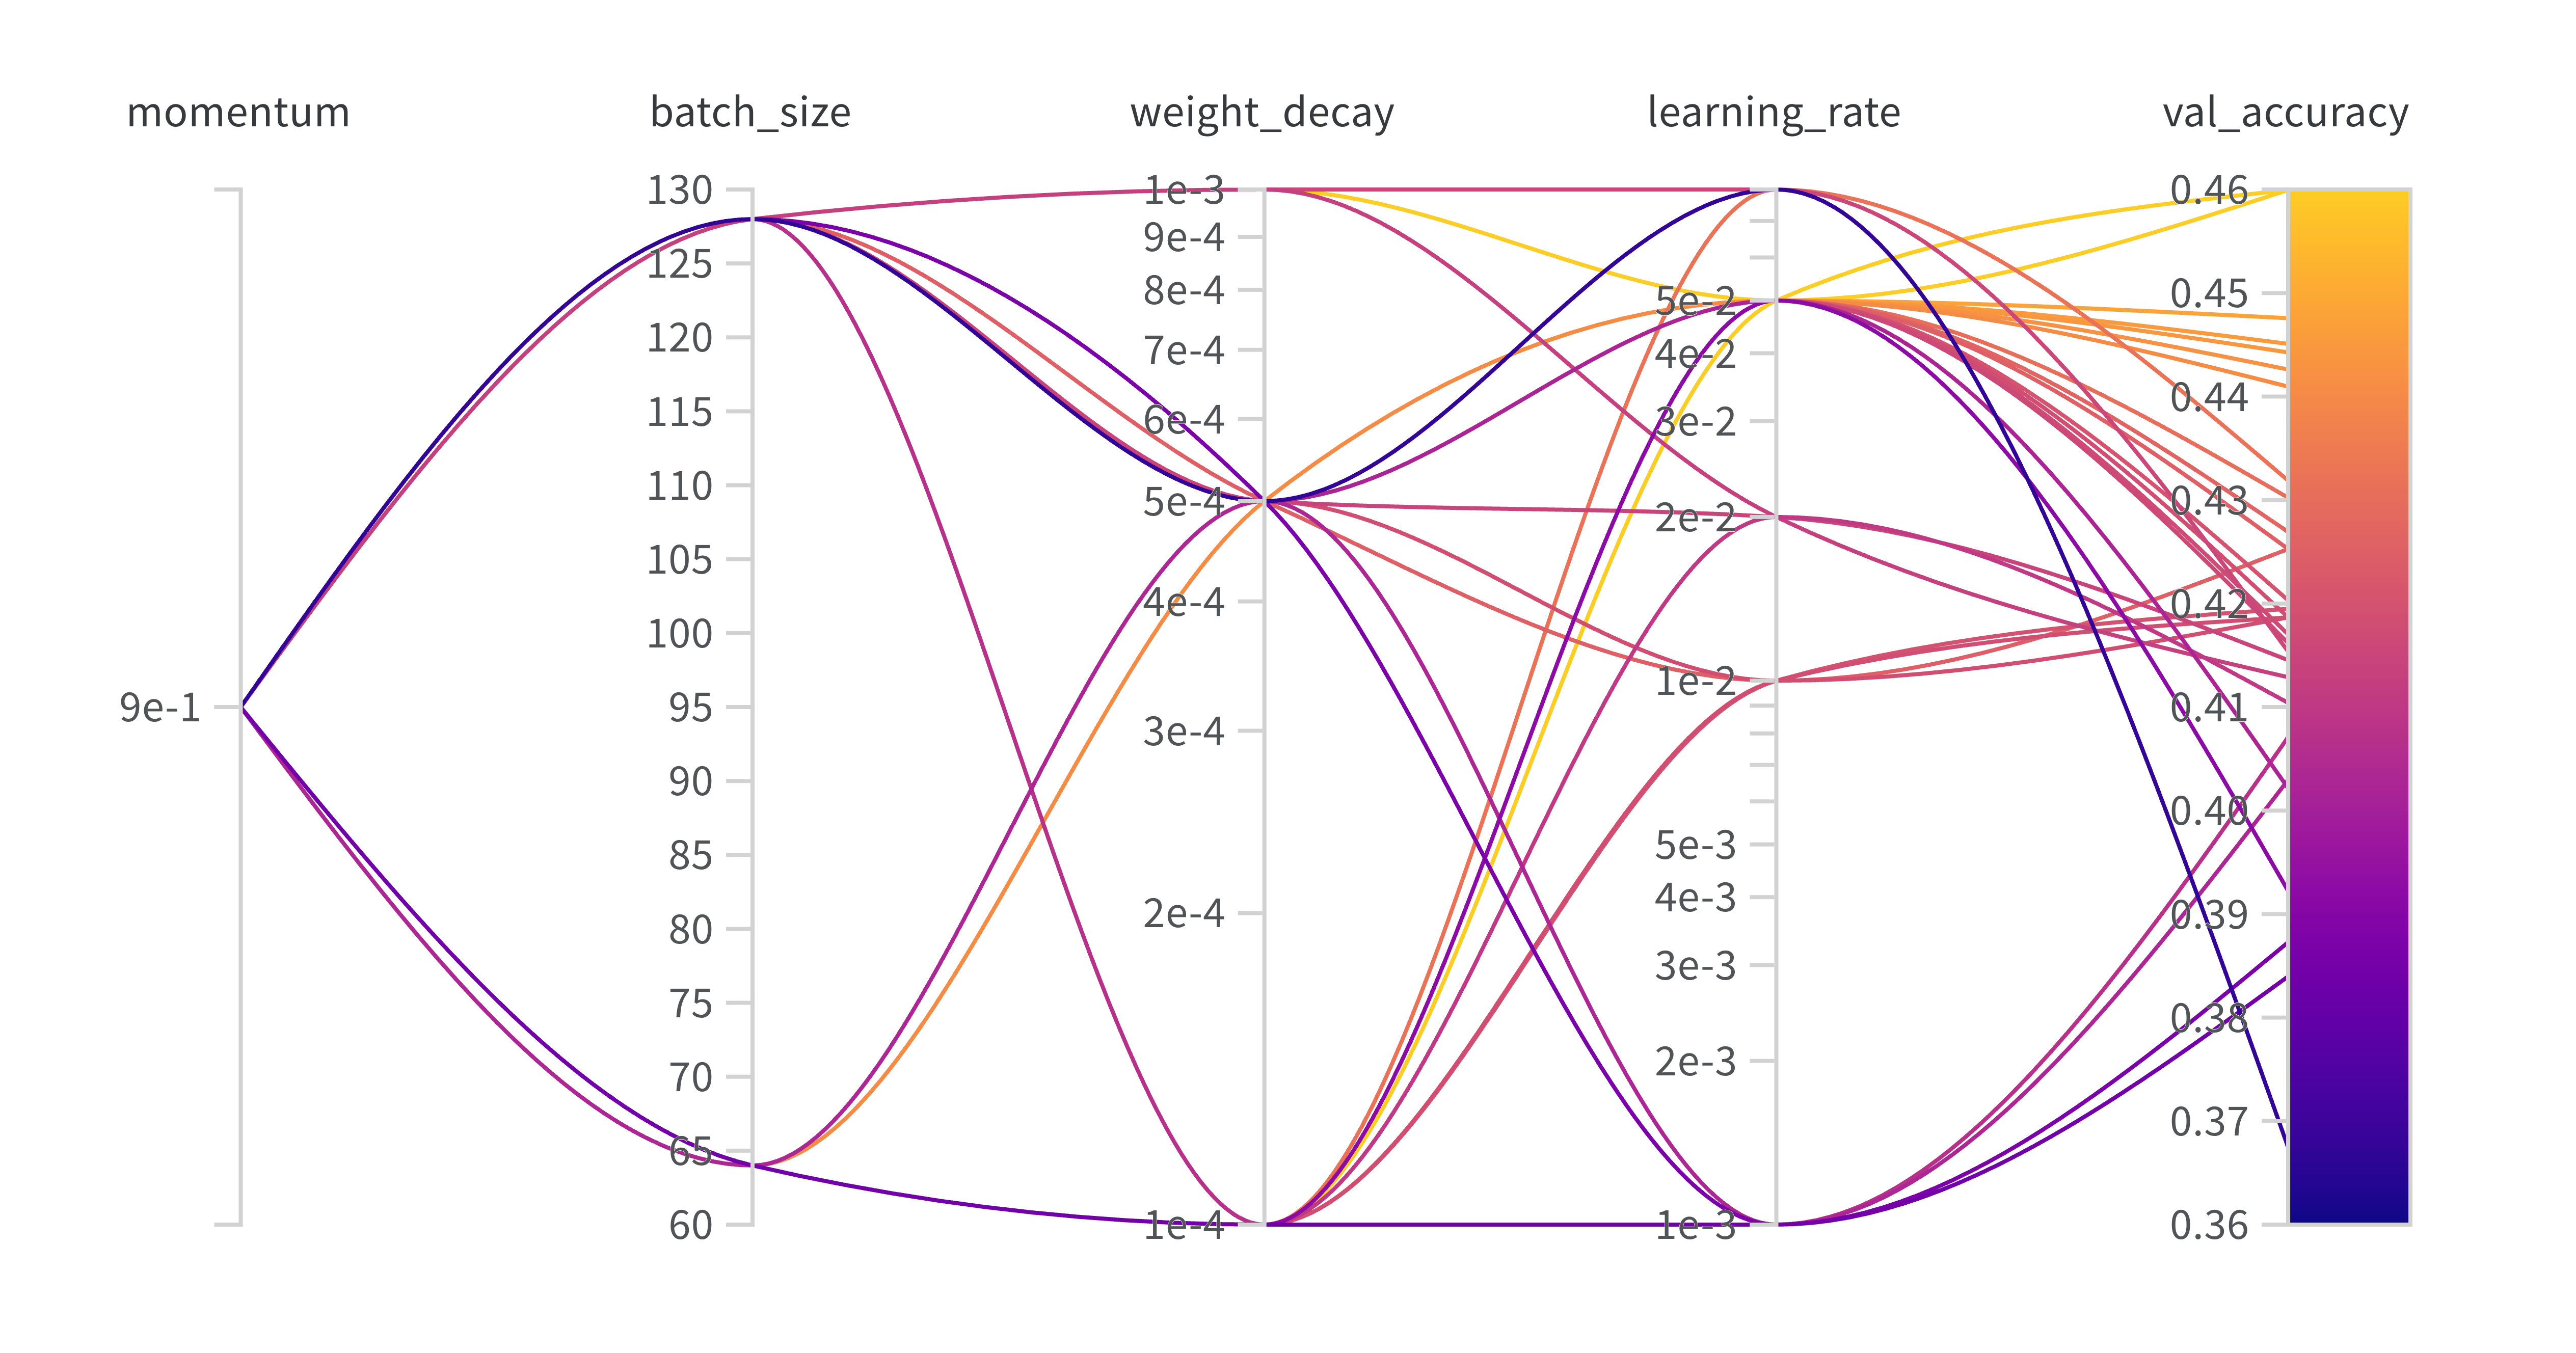
\includegraphics[width=1\linewidth]{figures/mufac-hyperparameter-tuning.png}
    \caption{MUFAC Hyperparmeter tuning for Resnet18}
    \label{fig:hyperparameterTuning2}
\end{figure}

\end{document}
